\documentclass[12pt]{article}
 
\usepackage[margin=1in]{geometry} 
\usepackage{amsmath,amsthm,amssymb}
\usepackage{hyperref}
\usepackage{graphicx}
\usepackage{xcolor}
\usepackage[many]{tcolorbox}
\tcbuselibrary{listings}
\usepackage{listings}

\definecolor{lg}{HTML}{f0f0f0}

\newtcblisting{pycode}{
    colback=lg,
    boxrule=0pt,
    arc=0pt,
    outer arc=0pt,
    top=0pt,
    bottom=0pt,
    colframe=white,
    listing only,
    left=15.5pt,
    enhanced,
    listing options={
        basicstyle=\small\ttfamily,
        keywordstyle=\color{blue},
        language=Python,
        showstringspaces=false,
        tabsize=2,
        numbers=left,
        breaklines=true
    },
    overlay={
        \fill[gray!30]
        ([xshift=-3pt]frame.south west)
        rectangle
        ([xshift=11.5pt]frame.north west);
    }
}

\lstset{
    language=Python,
    basicstyle=\small\ttfamily,
}


\begin{document}
 
\title{Exercise 6}
\author{Jari Mattila - 35260T\\
ELEC-E8125 - Reinforcement Learning}

\maketitle

\section*{Task 1}

The training performance plot for Task 1 is presented in Figure~\ref*{fig:fig1} for the continuous Cartpole environment. 
The variance learned as a parameter of the network is applied and TD(0) updates are performed at the end of each episode.
\newline

\noindent
Source files: cartpole\_task1.py, agent.py

\begin{figure}[phb] 
	\centering  % Remember to centre the figure
    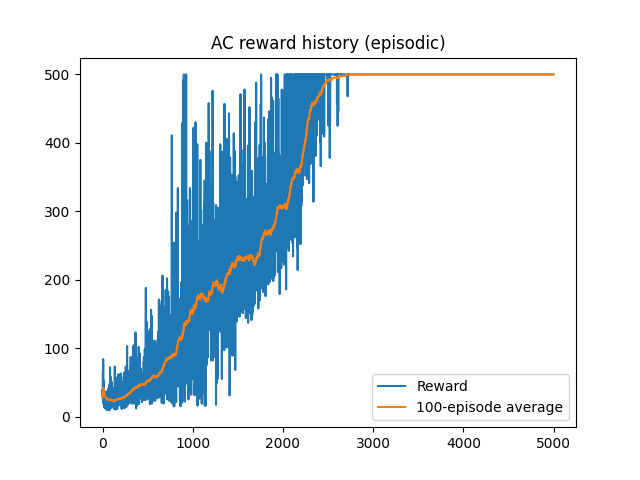
\includegraphics[width=0.9\columnwidth]{img/Figure_1_task_1_cumulative_reward.png}
	\caption{Training performance using an episodic version of actor-critic algorithm.}
	\label{fig:fig1}
\end{figure}

\pagebreak


\section*{Question 1}

What is the relationship between actor-critic and REINFORCE with baseline?
\newline

In the actor critic algorithm, the baseline in the REINFORCE with baseline method is replaced with the state value function that is updated along episodes by means of least squares over gathered data. 

\section*{Question 2}

How can the value of advantage be intuitively interpreted?
\newline

The value of advantage corresponds to the advantage of choosing a particular action $a$ over the current policy, i.e., how much better is taking action $a$ compared to average (see slide 12 of Lecture 6).


\section*{Task 2}

The training performance plot for Task 2 is presented in Figure~\ref*{fig:fig2}. 
The actor-critic algorithm was updated to perform TD(0) updates every 50 timesteps,
instead of updating the network at the end of each episode. 
\newline

\noindent
Source files: cartpole\_task2.py, agent.py

\begin{figure}[pht] 
	\centering  % Remember to centre the figure
    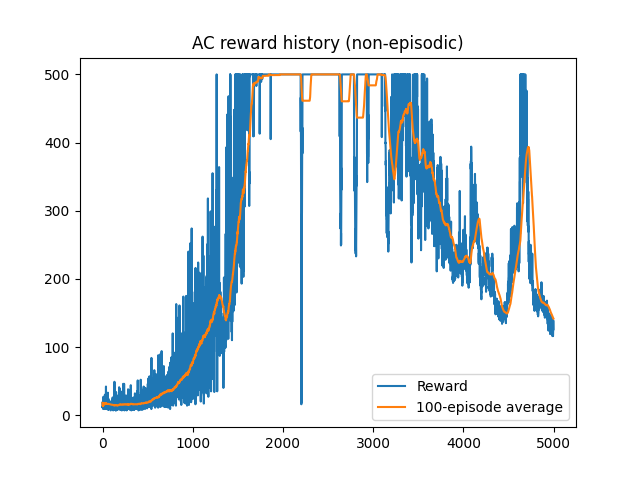
\includegraphics[width=0.8\columnwidth]{img/Figure_2_task_2_cumulative_reward.png}
	\caption{Training performance using a non-episodic version of actor-critic algorithm.}
	\label{fig:fig2}
\end{figure}

\begin{figure}[phb] 
	\centering  % Remember to centre the figure
    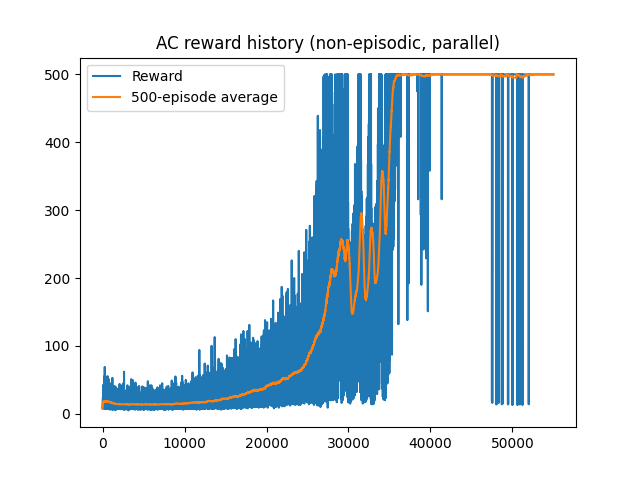
\includegraphics[width=0.8\columnwidth]{img/Figure_3_task_3_cumulative_reward_ContinuousCartPole-v0.png}
	\caption{Training performance using a non-episodic parallel version of actor-critic algorithm.}
	\label{fig:fig3}
\end{figure}


\section*{Task 3}

The training performance plot for Task 3 is presented in Figure~\ref*{fig:fig3}. The actor-critic algorithm was updated to use parallel data collection.
The training was executed using default parameters (8 processes, 8 envs per process) that correspond to 64 parallel environments. 
\newline

\noindent
Source files: parallel\_cartpole.py, agent.py

\pagebreak


\section*{Question 3}

How is parallel data collection different from the parallelism in
multiple\_cartpoles.py script we’ve seen in Exercises 1 and 5? Can it replace multiple runs of
the training algorithm for comparing RL algorithms? \textbf{Explain your answer.}
\newline

Several repetitions of the experiment are performed in the multiple\_cartpoles.py script, after which e.g. mean and variance can be calculated across all repetitions. 
In the parallel\_cartpole.py script, each worker generates experiences (i.e. state, next\_state, action\_prob, reward, done) that are combined with each time step. The agent updates its policy after every $N$ (=50) steps using the combined experiences. After that all workers continue to generate experiences with the updated parameters.
\newline

For example, if you want to compare the convergence properties (e.g. mean and variance) of RL algorithms, parallel data collection cannot replace multiple runs of the training algorithm.
Parallel data collection enables faster overall data collection and may reduce correlation in the collected data that can be beneficial for neural networks. Similar benefits can be achieved by experience replay within off-policy algorithms.



\section*{Question 4}

Figure 1 shows the training performance for all three actor-critic
variants and the REINFORCE algorithm from the last lecture. In terms of initial performance,
REINFORCE seems to completely outperform all tested A2C flavours on Cartpole, despite being
a simpler algorithm. \textbf{Why is it so? Explain your answer.}
\newline

In the REINFORCE with baseline algorithm, rewards were normalized to reduce variance and support gradient calculation. This was possible because rewards were collected throughout the episode before updates were applied. This could explain the better initial performance of the REFORCE algorithm compared to the AC algorithms as, e.g., the episodic AC algorithm does not exploit rewards that could be normalized. 


\section*{Question 5.1}

How do actor-critic methods compare to REINFORCE in terms of
bias and variance of the policy gradient estimation? \textbf{Explain your answer.}
\newline

In the episodic version of the AC algorithm, the baseline in the REINFORCE with baseline algorithm is replaced by the state value function that provides a smooth approximation of gathered data and thus lower variance for calculating the policy gradient. Adding a baseline to REINFORCE should not cause any bias (see slide 19 of lecture 5), thus bias is more related to using an episodic or non-episodic version of the algorithm.


\section*{Question 5.2}

How could the bias-variance tradeoff in actor-critic be controlled?
\newline

The episodic Monte Carlo (REINFORCE) methods provide high variance and zero bias, and non-episodic temporal difference (esp. TD(0)) methods provide low variance with some bias (see e.g. slide 9 of lecture 3). 
Changing the AC algorithm from the episodic version to a more non-episodic TD form, which updates the policy after every $N$ steps, provides less variance with some bias. 
Also, eligibility traces and TD($\lambda$) can be used to vary the bias-variance tradeoff between the Monte Carlo method and TD(0) (see Lecture 3 slides).  


\section*{Question 6}

What are the advantages of policy gradient and actor-critic methods
compared to action-value methods such as Q-learning? \textbf{Explain your answer.}
\newline

One advantage of policy gradient and actor-critic methods is that they can handle large and continuous action spaces that can only be discretized with action value methods (such as Q-learning).
Another advantage is the handling of stochastic policies that are required in environments where the optimal policy is stochastic and, e.g., requires the use of probability distributions.


\nocite{*}


\bibliographystyle{ieeetr}
\bibliography{template}  % Modify template with your bibliography name
\end{document}
